\documentclass[kulak]{kulakarticle}

\usepackage{amsmath}
\usepackage{amssymb}
\usepackage{amsfonts} % for \mathbb
\usepackage{amsthm}
\usepackage{tcolorbox}
\usepackage{mathtools}
\usepackage{siunitx}
\usepackage{cancel}

\let\epsilon\varepsilon

\newcommand{\R}{\mathbb{R}} % Real numbers
\newcommand{\C}{\mathbb{C}} % Complex numbers
\newcommand{\Q}{\mathbb{Q}}
\newcommand{\N}{\mathbb{N}}

\sisetup{output-decimal-marker={.}}
\sisetup{separate-uncertainty=true}		% Dit is voor de plus-minus
\sisetup{per-mode=fraction}

\newcommand*\diff{\mathop{}\!\mathrm{d}}
\newcommand*\Diff[1]{\mathop{}\!\mathrm{d^#1}}

\DeclareSIUnit\biti{bit_i}
\DeclareSIUnit\symbool{symbool}
\DeclareSIUnit\symbolen{symbolen}
\DeclareSIUnit\combinatie{combinatie}
\DeclareSIUnit\baud{baud}
\newcommand{\sam}{\text{sam}}

\newcommand\numberthis{\addtocounter{equation}{1}\tag{\theequation}}

\newcommand{\rood[1]}{\color{red}#1\color{black}}

\usepackage[dutch]{babel}
\usepackage{hyperref}

\setlength{\parindent}{0pt}

%\usepackage{draftwatermark}
%\SetWatermarkText{\normalfont Vincent Van Schependom}
%\SetWatermarkAngle{30}
%\SetWatermarkScale{1.5}

\title{Oude examenvragen Informatieoverdracht en -verwerking}
\author{Vincent Van Schependom}
\date{Academiejaar 2024-2025}
\address{
	\textbf{Informatieoverdracht en -verwerking}\\
	Prof. Lieven De Lathauwer \& Ben Hermans}

\begin{document}

	\maketitle

	\section*{Inleiding}

	Dit document bevat alle examenvragen die tijdens de hoorcolleges van het vak \textit{Informatieoverdracht en -verwerking} werden aangehaald door professor De Lathauwer (A1 t.e.m. A4) en Ben Hermans (de rest). Ik typte ook de oplossingswijze uitgebreid uit. De uitkomsten zijn zeker correct, aangezien de eindoplossingen aan bord werden gebracht of mondeling werden meegedeeld tijdens de les. Tip voor toekomstige studenten: ga zeker naar de les en laat dit vak niet liggen tot in de blok. Veel plezier ermee!

	\section{Discrete informatiebronnen}

	\subsection{Hoeveelheid informatie \& efficiëntie}

	In de studierichting Ingenieurswetenschappen hebben studenten de keuze uit mogelijkheden \(A, B, C\) en \(D\) voor hun hoofd- en nevenrichting, zoals te zien is in Tabel \ref{tab:mogelijkheden}.

	\begin{table}[h!]
		\centering
		\begin{tabular}{l | l | l}
		Hoofdrichting & Nevenrichting & \% studenten \\ \hline
		A & B & 40 \\
		A & C & 30 \\
		B & C & 20 \\
		B & D & 10
		\end{tabular}
		\caption{Voorkomende combinaties [maior,minor] met hun bijhorende kans.}
		\label{tab:mogelijkheden}
	\end{table}

	Gemiddeld gaat 80\% van de studenten verder in zijn/haar hoofdrichting; 20\% gaat verder in zijn/haar nevenrichting.\\

	\underline{Gevraagd}:
	\begin{enumerate}
		\item Wat is de gemiddelde hoeveelheid informatie \(H(A)\)?
		\item Hoeveel info geeft de Master-keuze nadat de Bachelor-keuze geweten is?
		\item Wat is de waarschijnlijkheidsredundantie \(R_w\) voor optredende Bachelor-Master combinaties?
	\end{enumerate}

	\hfill \\
	\underline{Oplossing}:
	\begin{enumerate}
		\item \( \text{Ba}=\{ [A,B], [A,C], [B,C], [B,D] \} \) is de verzameling van voorkomende Bachelor-keuzes. Dan is de gemiddelde hoeveelheid informatie: \[ H(\text{Ba})= - \sum_{i=1}^{4} p_i \log{p_i} = \boxed{\SI{1.846}{\biti \per \combinatie}} \]

		\item \( \text{Ma}=\{ A,B,C,D \} \) is de verzameling van voorkomende Master-keuzes.
		We gebruiken de voorwaardelijke hoeveelheid informatie voor de Master-keuze nadat de keuze in de Bachelor gekend is: \begin{align*}
			H(\text{Ma}\mid \text{Ba}) &= -\sum_{\text{Ba}=[A,B]}^{[B,D]}\sum_{\text{Ma}=A}^{D} P(\text{Ba})\cdot P(\text{Ma}\mid \text{Ba})\cdot \log{P(\text{Ma}\mid \text{Ba})} \\
			&= ... \\
			&= \boxed{\SI{0.7219}{\biti \per student}}
		\end{align*}

		\item We maken alle mogelijke Bachelor-Master combinaties en zien dat we \(\#\text{Ba} \cdot \#\text{Ma} = 8\) mogelijkheden hebben. De hoeveelheid informatie zou maximaal zijn voor gelijke kansen, d.w.z. voor \(p=1/8\). De maximale hoeveelheid informatie, \(\max H(\text{Ba}, \text{Ma})\), is dan \(\log{8}\) ofwel \(\SI{3}{\biti \per student}\). Voor de effectieve hoeveelheid informatie die wordt doorgegeven vinden we \[H(\text{Ba}, \text{Ma}) = H(\text{Ba}) + H(\text{Ma} \mid \text{Ba}) = \SI{2.5679}{\biti \per student} \] Aan de hand hiervan kunnen we \(R_w = 1 - \frac{H(\text{Ba}, \text{Ma})}{\max H(\text{Ba}, \text{Ma})} = \boxed{0.144}\) uitrekenen.
	\end{enumerate}

	\subsection{Broncodering}

	We beschouwen nu de gecombineerde gegevens [Ba, Ma].

	\hfill \\
	\underline{Gevraagd}:
	\begin{enumerate}
		\item Codeer de combinaties aan de hand van een Huffman-code.
		\item Wat is de gemiddelde codewoordlengte voor je broncodering?
		\item Bereken ook de efficiëntie.
	\end{enumerate}

	\hfill \\
	\underline{Oplossing}:
	\begin{enumerate}
		\item Bereken de kansen voor elke combinatie door de kansen van de Bachelor-keuze te vermenigvuldigen met de kans op een Master-keuze van 1) de maior en 2) de minor (aan de hand van de respectievelijke percentages 80\% en 20\%). Rangschik van meest waarschijnlijk (bovenaan) naar minst waarschijnlijk (onderaan) en doorloop het Huffman-procédé.

		Het bronalfabet is hier \[A=\{[AB,A],[AB,B],...,[BD,D]\}\] en het broncodealfabet is hier \[ B=\{1,0\} \] Na het bepalen van de Huffman-code vinden we een verzameling codewoorden \[ \boxed{C=\{00,10,11,0100,0101,0110,01110,01111\}} \] waarbij de codewoorden \(c_i\) elk een lengte \(l_i\) hebben. Aangezien elk codewoord 1 op 1 correspondeert met een symbool \(a_i\) uit het bronalfabet \(A\), en omdat bovendien \(\#A=n=8\), is ook \(\#C=8\) en dus \(i \in \{1,...,n=8\}\).

		\item We berekenen de gemiddelde codewoordlengte \(L\) van codewoorden \(c_i\) uit \(C\): \[ L=\sum_{i=1}^{8}p_il_i = \boxed{\SI{2.62}{symbolen/codewoord}} \]Aangezien een binair broncodealfabet slechts 2 symbolen (0 en 1) bevat (i.e. \(r=\#B=2\)), kunnen we dit ook interpreteren als \[L=\SI{2.62}{symbolen/codewoord}=\SI{2.62}{bit\per student}=2.62 \text{ binary digits per student} \]

		\item De efficiëntie van deze codering is \[\epsilon = \frac{H(A)}{L\cdot \log{r}}
		= \frac{\SI{2.568}{\biti \per symbool}}{\SI{2.62}{symbolen \per codewoord}\cdot \SI{1}{bit \per symbool}} = \boxed{98\%} \]
	\end{enumerate}

	\newpage

	\section{Continue informatiebronnen}

	Beschouw volgende twee muzieksignalen, beiden mono-signaal aan een frequentie van 0-\SI{5}{\kilo \hertz}:
	\begin{itemize}
		\item \textit{Signaal 1}: Gaussiaans verdeeld met \( \sigma=0.08 \)
		\item \textit{Signaal 2}: uniform verdeeld in het interval \( [-A,+A] \), met de grootte van \( A \) zó dat dit signaal hetzelfde vermogen heeft als \textit{Signaal 1}.
	\end{itemize}


	\underline{Gevraagd}:
	\begin{enumerate}
		\item Bereken het verschil in gemiddelde hoeveelheid informatie.
		\item Digitaliseer \textit{Signaal 2} door het te
		\begin{itemize}
			\item \underline{bemonsteren}: maak gebruik van de ir-vuistregel.
			\item \underline{kwantiseren}: bepaal het aantal intervallen \( K \), zodat dit een macht van 2 is en zodat de gemiddelde signaal-tot-kwantisatieruis \underline{\textbf{vermogens}}verhouding minstens \SI{100}{\decibel} bedraagt.
		\end{itemize}
		\begin{enumerate}
			\item[a)] Wat is het informatiedebiet?
			\item[b)] Wat is het transmissiedebiet?
		\end{enumerate}
	\end{enumerate}

	\underline{Oplossing}:

	\begin{enumerate}
		\item \textit{Signaal 1} is Gaussisch verdeeld, dus heeft een vermogen van \( P_{{X_1}} = \sigma^2 \).
		\textit{Signaal 2} is uniform verdeeld tussen \( [-A,+A] \) en heeft een vermogen van
		\begin{equation*}
			\begin{split}
				P_{{X_2}} & = \int_{-\infty}^{+\infty}x^2\cdot p(x) \diff{x} \\
				       & = \int_{-A}^{+A}x^2\cdot \frac{1}{2A} \diff{x} \\
				       & = \frac{1}{2A} \left[\frac{1}{3}A^3\right]^{+A}_{-A} \\
				       & = \frac{1}{6A} \left((+A)^3-(-A)^3\right) \\
				       & = \frac{A^2}{3}
			\end{split}
		\end{equation*}
		Omdat het vermogen van \textit{Signaal 1} gelijk moet zijn aan het vermogen van \textit{Signaal 2}, moet gelden dat
		\begin{equation*}
			\begin{split}
				P_{{X_1}} = P_{{X_2}} & \Leftrightarrow \sigma^2 = \frac{A^2}{3} \\
				& \Leftrightarrow 0.08^2 = \frac{A^2}{3} \\
				& \Leftrightarrow A = \sqrt{0.08^2\cdot 3} \approx 0.1386 \\
			\end{split}
		\end{equation*}
		Zo vinden we de gemiddelde hoeveelheid informatie die geleverd wordt door beide bronnen:
		\begin{align*}
			&H(X_1) = \log_2({\sigma\sqrt{2\pi e}}) &= \boxed{\SI{-1.597}{\biti \per bemonstering}} \\
			&H(X_2) = \log_2({2A}) &= \boxed{\SI{-1.851}{\biti \per bemonstering}}
		\end{align*}

		Het verschil bedraagt \boxed{\SI{0.254}{\biti \per bemonstering}}.

		\newpage

		\item We digitaliseren \textit{Signaal 2}:
		\begin{itemize}
			\item \underline{Bemonstering}:

			De bandbreedte (=maximale frequentie) bedraagt \( B =f_m= \) \SI{5}{\kilo\hertz}. Het bemonsteringstheorema van Nyquist zegt ons dat we een signaal foutloos kunnen reconstrueren als \( f_s \geq 2f_m \). De ingenieursvuistregel bouwt wat marge in en neemt de samplingfrequentie gelijk aan \( f_s=2.2f_m \).

			Voor dit signaal nemen we dus \[ f_s = 2.2\cdot \SI{5}{\kilo\hertz}=\boxed{\SI{11}{\kilo\hertz}} \]
			\item \underline{Kwantisatie}:

			De gemiddelde signaal-ruisverhouding moet ten minste \SI{100}{\decibel} bedragen. We zoeken \(K=2^n\) zodat geldt dat
			\begin{equation}
				\left(\frac{S}{N}\right)_0=K^2-1\geq \SI{100}{\decibel} \label{ongel1}
			\end{equation}

			We kunnen dit ook uitdrukken in decibel (\SI{}{\decibel}), en wel als volgt: \[\SI{}{\decibel}\left(\frac{S}{N}\right)_0 = 10\cdot \log_{10}\left(\left(\frac{S}{N}\right)_0\right) = 10 \cdot \log_{10}(\text{vermogensverhouding})\] Of nog: het aantal decibel is gelijk aan 10 keer de \( \log_{10} \) van een \underline{\textbf{vermogens}}verhouding (er wordt inderdaad gevraagd naar een vermogensverhouding, voor de amplitudeverhouding is het maal 20). We vatten de omzetting samen:
			\begin{equation*}
				\begin{split}
					\text{dB} &= 10 \cdot \log_{10}(\text{vermogensverhouding}) \\
					&= 10 \cdot \log_{10}(\text{amplitudeverhouding}^2) \\
					&= 20 \cdot \log_{10}(\text{amplitudeverhouding})
				\end{split}
			\end{equation*}

			We zoeken nu vanuit deze waarde van \SI{100}{\decibel} de overeenkomstige vermogensverhouding:
			\begin{equation*}
				\begin{split}
					10 \cdot \log_{10}(\text{vermogensverhouding}) = \SI{100}{\decibel} &\Leftrightarrow \log_{10}(\text{vermogensverhouding}) = \SI{10}{\decibel} \\
					& \Leftrightarrow \text{vermogensverhouding} = 10^{10}
				\end{split}
			\end{equation*}

			We vinden dus een vermogensverhouding van \( \left(\frac{S}{N}\right)_0 = 10^{10} \). Dit is gelijk aan \( 10000 \) miljoen. Als we dit invullen in de ongelijkheid \ref{ongel1}, wordt de \textit{min 1} verwaarloosbaar en krijgen we dus:
			\begin{equation*}
				\begin{split}
					K^2\geq \SI{100}{\decibel} &\Leftrightarrow K^2 \geq 10^{10} \\
					& \Leftrightarrow K \geq 10^5 \\
					& \Leftrightarrow 2^n \geq 10^5 \\
					& \Leftrightarrow n \geq \log_2(10^5)\approx 16.6
				\end{split}
			\end{equation*}

			We nemen dus als exponent \(n=17\), zodat \( K=2^n=2^{17} \) en we zien inderdaad dat voldaan is aan de voorwaarde \( K^2-1\geq 10^{10} \), want \( K^2=2^{34} \approx \SI{1.7e10}{} \), wat duidelijk groter is dan \(10^{10}\) na de aftrekking van het getal 1.

			 Nu berekenen we de grootte van de kwantisatieintervallen: \[
			\Delta (=a) = \frac{2A}{K} = \dfrac{2\cdot 0.1386}{2^{17}} = 0.1386 \cdot 2^{-16}
			\]We berekenen vervolgens de gemiddelde hoeveelheid informatie per bemonstering na kwantisatie. Omdat we hier te maken hebben met een uniforme verdeling is \(p(x_i)\) overal gelijk, maar als dat niet zo zou zijn, kunnen we de som uit het formularium -- die loopt van \(i=1\) tot \(K\), en die dus heel veel termen kan bevatten -- vereenvoudigen door alles in functie van \(K\) uit te drukken.

			Bijvoorbeeld: \(1/3\) van de amplitudes heeft kans \(p_1\), \(1/6\) heeft kans \(p_2\) en \(1/2\) heeft kans \(p_3\). Dan kunnen we de som van \(K\) termen herleiden tot eentje van slechts \(3\) termen. Voor deze oefening krijgen we -- wegens de uniforme kansverdeling -- een makkelijke uitdrukking: \begin{align*}
				H(x^{\Delta}) &= - \sum_{i=1}^{K} p(x_i) \cdot \Delta \cdot \log(p(x_i)\cdot \Delta) \\
				&= - K \cdot \frac{1}{2A} \cdot \Delta \cdot \log\left(\frac{1}{2A} \cdot \Delta \right)\\
				& = - \cancel{K} \cdot \frac{1}{\cancel{2A}} \cdot \frac{\cancel{2A}}{\cancel{K}} \cdot \log\left(\frac{1}{\cancel{2A}} \cdot \frac{\cancel{2A}}{K} \right)\\
				&= -\log\left(\frac{1}{K}\right)\\
				&= \SI{17}{\biti \per bemonstering}
			\end{align*}

			Dit stemt overeen met de approximatie:
			\[
			H(x^{\Delta}) \approx H(x)-\log_2(\Delta) = \SI{17}{\biti \per bemonstering}
			\]

			Aan de hand van \( H(x^{\Delta}) \) kunnen we nu het \underline{informatiedebiet} uitrekenen: \begin{align*}
				H_{t}(x^{\Delta}) &= 2B \cdot H(x^{\Delta}) \\
				&= \boxed{\SI{170}{\kilo \bit \per \second}} \\
				&\neq f_s \cdot H(x^{\Delta}) \text{ want we bereiken een maximum!}
			\end{align*}

			Voor \( K \) intervallen of niveaus hebben we \( n_q=\log_2(K) \) binary digits (bits) nodig. Het \underline{transmissiedebiet} is gelijk aan de frequentie waaraan we samplen, vermenigvuldigd met deze hoeveelheid bits. We vinden dat dit transmissiedebiet gelijk is aan \begin{align*}
				r_b &= f_s \cdot \log_2(K) \\
				&= \SI{11}{\kilo\hertz} \cdot \SI{17}{\bit} \\
				&= \boxed{\SI{187}{\kilo\bit\per\second}}
			\end{align*}

		\end{itemize}


	\end{enumerate}

	\newpage
	\section{Filters}


	\underline{Gevraagd} \\

	Ontwerp een laagdoorlaatfilter met minimale vertraging (hoogstens \SI{0.8}{\milli\second}) en maximale stopbandverzwakking -- waarvan de laatste geprioriteerd dient te worden, gegeven volgende zaken:

	\begin{itemize}
		\item De bemonsteringsfrequentie bedraagt \(f_{\text{sam}}=\SI{100}{\kilo\hertz}\)
		\item De doorlaatfrequentie bedraagt \(f_p=\SI{20}{\kilo\hertz}\)
		\item De stopfrequentie \(f_s\) ligt ergens tussen de \SI{20}{\kilo\hertz} en de \SI{23}{\kilo\hertz}
	\end{itemize}

	\underline{Oplossing}\\

	We beginnen met de eisen die we zeker weten. De \textit{lakse} voorwaarden behandelen we later. De \textbf{vertraging} \textbf{(die gelijk is aan de orde, \(M-1\), maal de sampling periode!)} moet sowieso minder dan \SI{0.8}{\milli\second} bedragen. We bepalen een \textbf{bovengrens} voor \(M\) (maar leggen nog geen waarde vast!):
	\begin{align*}
		(M-1) T_\sam \leq \SI{0.8}{\milli\second} &\Leftrightarrow \frac{(M-1)}{f_\sam}\leq \SI{0.8}{\milli\second} \\
		& \Leftrightarrow \frac{(M-1)}{\SI{100}{\kilo\hertz}}\leq \SI{0.8}{\milli\second} \\
		& \Leftrightarrow \frac{(M-1)}{10^5} \SI{}{\second}\leq \SI{0.8e{-3}}{\second} \\
		& \Leftrightarrow M-1 \leq \SI{0.8e2}{} = 80 \\
		& \Leftrightarrow M\leq81
	\end{align*}

	We berekenen de genormaliseerde frequenties:
	\begin{align*}
		\omega_p &= \frac{2\pi f_p}{f_\sam} = \frac{2\pi \cdot 20}{100} = \frac{2\pi}{5} \\
		\omega_s &= \frac{2\pi f_s}{f_\sam} \in \left[\frac{2\pi}{5},\frac{46\pi}{100}\right] = \left[\frac{2\pi}{5},\frac{23\pi}{50}\right]
	\end{align*}
	De transitieband is \(\omega_s-\omega_p\). Een \textbf{kleinere stopbandfrequentie \(f_s\)} (en dus ook \(\omega_s \downarrow\)) wil zeggen:
	\begin{itemize}
		\item[\(\rightarrow\)] Kleinere transitieband
		\item[\(\rightarrow\)] Grotere \(M\) nodig om dat te realiseren
		\item[\(\rightarrow\)] Grotere vertraging en meer energieverbruik (willen we niet!)
		\item[\(\rightarrow\)] Dus we nemen \(f_s\) zo \textbf{GROOT} mogelijk: \(f_s=\SI{23}{\kilo\hertz} \quad \Longrightarrow \quad \omega_s = \frac{23\pi}{50}\)
	\end{itemize}

	Uit \(\omega_p = \frac{20\pi}{50}\) en \(\omega_s = \frac{23\pi}{50}\) volgt dat de breedte van de transitieband gelijk is aan \[\omega_s-\omega_p=\frac{23-20}{50}\pi = \frac{3\pi}{50}\]	We gaan nu op zoek naar de correcte vorm van het window. Hiervoor zoeken we \(X\) zodat \[\frac{3\pi}{50}=\frac{X}{M} \Leftrightarrow \frac{50X}{3\pi}=M\] We berekenden al dat het aantal samples \(M\) maximum 81 mag zijn. We kunnen dus een bovengrens voor \(X\) bepalen:
	\begin{align*}
		M \leq 81 & \Leftrightarrow \frac{50X}{3\pi} \leq 81 \\
					& \Leftrightarrow 50X \leq 81 \cdot 3\pi \\
					& \Leftrightarrow X \leq 15.27
	\end{align*}

	We kiezen voor het \textbf{Hamming} window, omdat dit het window is met de grootste stopbandverzwakking \(\delta_s\) (zoals gevraagd), die voldoet aan de voorwaarde \(X \leq 15.27\). We berekenen nu de waarde die we nodig hebben voor \(M\) (en hopen dat die effectief kleiner is dan 81):
	\begin{equation*}
		\frac{3\pi}{50} \overset{\text{Hamming}}{=} \frac{15.14}{M} \quad \Leftrightarrow \quad M \approx 80.32
	\end{equation*}

	We ronden deze waarde af \textbf{naar boven} en vinden een (oneven!) waarde van \(M=\boxed{81}\). Het is noodzakelijk dat deze waarde \textbf{oneven} is, zodat we steeds mooi rond 0 samplen.


	\newpage \section{Discrete transmissiekanalen}

	Een bron zendt (alle mogelijke) pakketjes uit van telkens twee bits. De foutkans voor elk afzonderlijk symbool bedraagt 1\% en is onafhankelijk van een ander symbool. De kans op het doorsturen van een 0 of een 1 is even waarschijnlijk.

	\hfill \\
	\underline{Gevraagd}:
	\begin{enumerate}
		\item Bepaal de kanaalmatrix \(Q\), \(H(X), H(Y), H(X\mid Y)\) en \(H(Y\mid X)\)
		\item Wat is de gemiddelde symboolfoutkans?
		\item Het team onderzoekers dat de bron bestudeert, vindt de foutkans te groot en gaat kanaalcodering toepassen aan de hand van een \((n,k)\) systematische lineaire blokcode met generatormatrix \[
		G=\begin{bmatrix}
		1 & 0 & 1 & 1 & 0 \\
		0 & 1 & 1 & 0 & 1 \\
		\end{bmatrix}=\begin{bmatrix}
		\mathbb{I}_{k} & P_{k\times (n-k)}
	\end{bmatrix} \quad \text{met } n=5, k=2\]Wat is de coderingsefficiëntie \(\varepsilon\)? Bepaal de minimumafstand \(d_{\text{min}}\), het foutdetectievermogen \(e\) en het foutcorrectievermogen \(t\) van de blokcode.
		\item Hoe groot is de kans op een niet-corrigeerbare fout bij het doorsturen van een codewoord? \textit{Tip:} de kans dat er exact \(x\) symbolen fout zijn in een serie van \(y\) bits is \(\binom{y}{x}p^x(1-p)^{y-x}=\frac{y!}{x!(y-x)!}\)
	\end{enumerate}

	\hfill \\
	\underline{Oplossing}:
	De matrix met bronvectoren is \[
	X=\begin{bmatrix}
		0 & 0 \\
		0 & 1 \\
		1 & 0 \\
		1 & 1
	\end{bmatrix}\]
	en de foutkansen voor beide symbolen (0 en 1) zijn gelijk, namelijk \(p=0.01\).

	\begin{enumerate}
		\item De kanaalmatrix \(Q\) geeft bevat alle kansen \(q_{ji}=q(y_j \mid x_i)\), i.e. de kans dat een symbool \(y_j\) wordt ontvangen als een symbool \(x_i\) werd verzonden. De kolommen van deze matrix sommeren naar 1, want per verzonden symbool \(x_i\) wordt er sowieso een symbool \(y_j\) ontvangen. We vinden dat \[
		Q = \begin{bmatrix}
			a & b & b & c \\
			b & a & c & b \\
			b & c & a & b \\
			c & b & b & a
		\end{bmatrix}\] waarbij \begin{align*}
		 a &= P(\text{symbool juist ontvangen}) \cdot P(\text{symbool juist ontvangen}) &=&\, 0.99^2 &&\\
		 b &= P(\text{symbool juist ontvangen}) \cdot P(\text{symbool fout ontvangen}) &=&\, 0.99 \cdot 0.01&&\\
		 c &= P(\text{symbool fout ontvangen}) \cdot P(\text{symbool fout ontvangen}) &=&\, 0.01^2&&
		\end{align*}
		We mogen de kansen gewoon vermenigvuldigen, want de foutkansen zijn onafhankelijk.

		Omdat 0 en 1 met gelijke kans voorkomen, weten we dat \(\forall x \in \{00,01,10,11\} : p(x)=\left(\frac{1}{2}\right)^2\). \\We kunnen dus berekenen dat \[
		H(X)=-\sum_{i=1}^4 p(x_i) \log(p(x_i))=-4 \cdot \left( 0.5^2 \cdot \log(0.5^2) \right) = \boxed{\SI{2}{\biti \per \symbool}} \]

		We berekenen nu de voorwaardelijke hoeveelheid informatie \(H(Y \mid X)\). Merk op dat de kolomsommen van \(Q\) over \(q_{ji} \cdot \log(q_{ji})\) telkens dezelfde zijn en dat ook \(p(x_1)=...=p(x_4)\).
		\begin{align*}
			H(Y \mid X) &= - \sum_{i=1}^{4} \sum_{j=1}^{4} p(x_i) \cdot q_{ji} \cdot \log(q_{ji})\\
					&= - \sum_{i=1}^{4} p(x_i) \sum_{j=1}^{4} q_{ji} \cdot \log(q_{ji})\\
					&= - \cancel{4} \cdot \left[ \cancel{\left(\frac{1}{2}\right)^2} \cdot \left(0.99^2 \cdot \log(0.99^2) + 2 \cdot 0.99 \cdot 0.01 \cdot \log(0.99 \cdot 0.01) + 0.01^2 \cdot \log (0.01^2)\right) \right] \\
					&= \boxed{\SI{0.1616}{\biti \per \symbool}}
		\end{align*}

		We kunnen \(H(Y)\) uitrekenen aan de hand van de formule, maar we kunnen dit ook beredeneren. Niet alleen de kanaalmatrix, maar ook de foutkansen (i.e. de ruis), zijn symmetrisch. We kunnen dus direct inzien dat elke \(q(y_j) = 0.25\). Dit wil zeggen dat \(H(X)=H(Y)\). Een andere manier om dit te bekijken: \begin{align*}
			\begin{bmatrix}
				\vdots \\
				q(y_j) \\
				\vdots
			\end{bmatrix} = Q \cdot \begin{bmatrix}
			\vdots \\
			p(x_i) \\
			\vdots
			\end{bmatrix}
		\end{align*}

		Omdat we nu weten dat \(H(X)=H(Y)\), volgt uit \begin{align*}
			R&=H(X)-H(X \mid Y)\\&=H(Y)-H(Y\mid X)
		\end{align*} dat ook \(H(X\mid Y)=H(Y\mid X)=\SI{0.1616}{\biti \per \symbool}\).

		\item We berekenen de gemiddelde symboolfoutkans, die hetzelfde is bij zonder en ontvanger, omdat \(Q \in \R^{4\times 4}\) een vierkante matrix is.
		\begin{align*}
			P_e &= \sum_{j=1}^{4}q(y_j)\cdot p(e\mid y_j)\\
				&= \sum_{j=1}^{4}q(y_j)\cdot [1-p(x_j\mid y_j)]\\
				&= \cancel{4} \cdot\cancel{ \left(\frac{1}{2}\right)^2} \cdot (1-q_{11}^2)\\
				&= 1-0.99^2\\
				&\approx \boxed{2\%}
		\end{align*}

		\item De coderingsefficiëntie van de \((n,k)=(5,2)\) blokcode bedraagt \[\varepsilon = \frac{k}{n}=\frac{2}{5}=\boxed{0.4}\] Door de bronvectoren \(U_i = [0 \, 0],[0 \, 1],[1 \, 0], [1 \, 1] \in \R^k\) te vermenigvuldigen met de generatormatrix \(G\), verkrijgen we codevectoren \(C_i\). Omdat \([0 \, 0]\) een bronvector is, zal de kleinste hammingafstand \(d_{\text{min}}\) gewoonweg gelijk zijn aan het kleinste gewicht \(g\) (i.e. het aantal enen) van alle de codewoorden.

		We kunnen nu zonder veel rekenwerk de matrix opstellen, die in de rijen de codevectoren \(C_i\in \R^n\) bevat. Merk op: de eerste twee kolommen bevatten sowieso de bronvectoren, want de lineaire blokcode is \textbf{systematisch}: de \(k\) symbolen \(u_i\), gegenereerd door de bron, komen voor als eerste \(k\) symbolen in het codewoord na kanaalcodering.
		\newpage
		Snelle manier om de matrix \[\begin{bmatrix}
			0 & 0 & 0 & 0 & 0 \\
			0 & 1 & 1 & 0 & 1 \\
			1 & 0 & 1 & 1 & 0 \\
			1 & 1 & 0 & 1 & 1
		\end{bmatrix}\] met codevectoren te vinden:
		\begin{itemize}
			\item Kolom 1 en 2 bevatten als eerste \(k=2\) symbolen de bronvectoren \(U_i\).
			\item Rij 1 bevat enkel nullen.
			\item Rij 2 bevat de tweede rij uit \(P\).
			\item Rij 3 bevat de eerste rij uit \(P\).
			\item Rij 4 bevat de som van de eerste twee rijen uit de \(P\), \textbf{modulo 2}.
		\end{itemize}

		We zien meteen dat \(d_{\text{min}}=3\), omdat het laagste gewicht van een codevector, verschillend van de nulvector, gelijk is aan 3. Het bepalen van het foutdetectievermogen \(e\) en het foutcorrectievermogen \(t\) is kinderspel: \[e=d_{\text{min}}-1=\boxed{2} \qquad \text{en} \qquad t=\left\lfloor\frac{d_{\text{min}}-1}{2}\right\rfloor=\boxed{1}\]

		\item Omdat het foutcorrectievermogen gelijk is aan \(t=1\), treedt een niet-corrigeerbare fout op indien er meer dan 1 bit fout is. We vinden dus dat \begin{align*}
			P_e &= 1 - p(\text{1 bit fout}) - p(\text{0 bits fout}) \\
			&= 1- \rood[p(\text{bit}_1 \text{ fout}) - \ldots - p(\text{bit}_5 \text{ fout}) ] - p(\text{alle bits juist})\\
			&= 1 - \left(\rood[5] \cdot 0.01 \cdot 0.99^4\right) - \left(0.99^5\right) \\
			&= \boxed{0.098\%}
		\end{align*}
		We verkleinen de foutkans dus met factor 2 door aan kanaalcodering te doen. Omdat we nu extra bits versturen, zal ook het netto transmissiedebiet \( r_b \) dalen.
	\end{enumerate}

	\newpage

	\section{Geleide fysische transmissie}

	In 1956 werd de eerste transatlantische coaxiale kabel in gebruik genomen. Hij functioneerde gedurende 20 jaar zonder noemenswaardige defecten en transporteerde 36 telefoonkanalen in de frequentieband van 20 tot 170 kHz. Deze frequentieband werd opgelegd door de mogelijkheden van de versterkers die waren uitgevoerd met radiobuizen en die een vermogenversterking van 60 dB realiseerden in de opgegeven frequentieband.

	\hfill \\
	\underline{Gevraagd:}
	Gegeven de transmissielijnparameters \begin{align*}
			R &= \SI{2e-5}{\ohm/\kilo\meter} &\text{weerstand}\ &= \text{verlieselement} \\
			L &= \SI{0.25e-3}{H/\kilo\meter} &\text{inductantie} &= \text{hoeveelheid opgeslagen magnetische energie} \\
			C &= \SI{4e-8}{F/\kilo\meter} &\text{capaciteit} &= \text{hoeveelheid opgeslagen elektrische energie} \\
			G &= \SI{3e-3}{S/\kilo\meter} &\text{conductantie} &= \text{`verliesstroom' = verlieselement}
		\end{align*} Bereken voor de grootste frequentie van \SI{170}{\kilo\hertz} de maximale afstand tussen de versterkers zodat de verzwakking van het signaal telkens gecompenseerd werd.

	\hfill \\
	\underline{Oplossing:}
	We berekenen de propagatieconstante \begin{align*}
		\gamma &= \sqrt{(R+j\omega L)(G+j\omega C)} \\
				&= \sqrt{(R+j \cdot 2\pi f \cdot L)(G+j \cdot 2\pi f \cdot C)} \\
				&= 0.11851 + 3.37984j
	\end{align*}
	De verzwakkingsconstante is dus gelijk aan \(\alpha = 0.11851\) en de faseconstante is gelijk aan \(\beta = 3.37984\). \\Nu geldt dat de verzwakking gelijk is aan \[
	A = 20 \cdot \log_{10} e^{\alpha \cdot 10^3 \unit{\meter}}=\alpha \cdot 10^3 \cdot 20 \cdot \log_{10} e \qquad \text{\textbf{(in dB per \underline{km}!)}}\] De verzwakking is kleiner dan of gelijk aan 60 dB als \(A \cdot l \leq \SI{60}{\decibel}\), ofwel als \[l\leq\frac{60}{0.11851\cdot 10^3\cdot 20 \cdot \log_{10} e} = \boxed{\SI{58}{\kilo\meter}}\]

\newpage
	\section{Ongeleide fysische transmissie}

	Een anonieme toerist ontdekte onlangs de verloren bibliotheek van Alexandrië.
	Een team van historisch aangelegde ingenieurs hebben hier wind van opgevangen en zijn van plan een missie te organiseren om alle informatie uit de bibliotheek over te brengen naar een veilige locatie. De hoeveelheid informatie schatten ze op ongeveer 3,6 Tbit (1 Tbit = \(10^{12}\) bit). De bandbreedte van hun overdracht
	zal 100 MHz bedragen op een draaggolf van 1 GHz. Voor hun missie hebben ze reeds de volgende infrastructuur:\begin{enumerate}
		\item[i. ] een paraboolantenne als zender met 1 kW zendvermogen, 1 m diameter en 80\% efficiëntie
		\item[ii. ] een satelliet op 1000 km afstand tot de zender, met 20 dB ontvangstwinst en 80 dB interne versterking (van het signaal, niet de ruis), die zelf signalen isotroop uitstraalt
		\item[iii. ] een paraboolantenne om het signaal op de veilige plaats te ontvangen, 1000 km van de satelliet, met een ontvangstwinst van 40 dB en een lokale (ruis)temperatuur van 293 K	\end{enumerate}

	De zendantenne kan niet rechtstreeks naar de ontvangstantenne stralen maar moet via de satelliet gaan.

	Omdat ze te veel aandacht zouden trekken als ze te lang op de locatie van de gevonden bibliotheek blijven, wensen ze de klus te klaren binnen één uur. De infrastructuur kan desnoods aangepast worden op de volgende drie manieren. \begin{enumerate}
		\item Een vergroting van de bandbreedte naar oneindig voor 20000 euro
		\item Een vergroting van de zendantenne aan 2000 euro per extra meter diameter
		\item Een verhoging van de winst van de ontvangstantenne aan 1000 euro per extra dB
	\end{enumerate}

	Verifieer of de huidige infrastructuur voldoende is om alle informatie in de gewenste tijd over te kunnen brengen en zo niet, bereken dan het bedrag dat het team van ingenieurs nog zal moeten spenderen.

	\hfill \\
	\underline{Oplossing} zie Figuur \ref{fig:satelliet} voor een schets van de gegevens.

	\begin{figure}[h!]
		\centering
		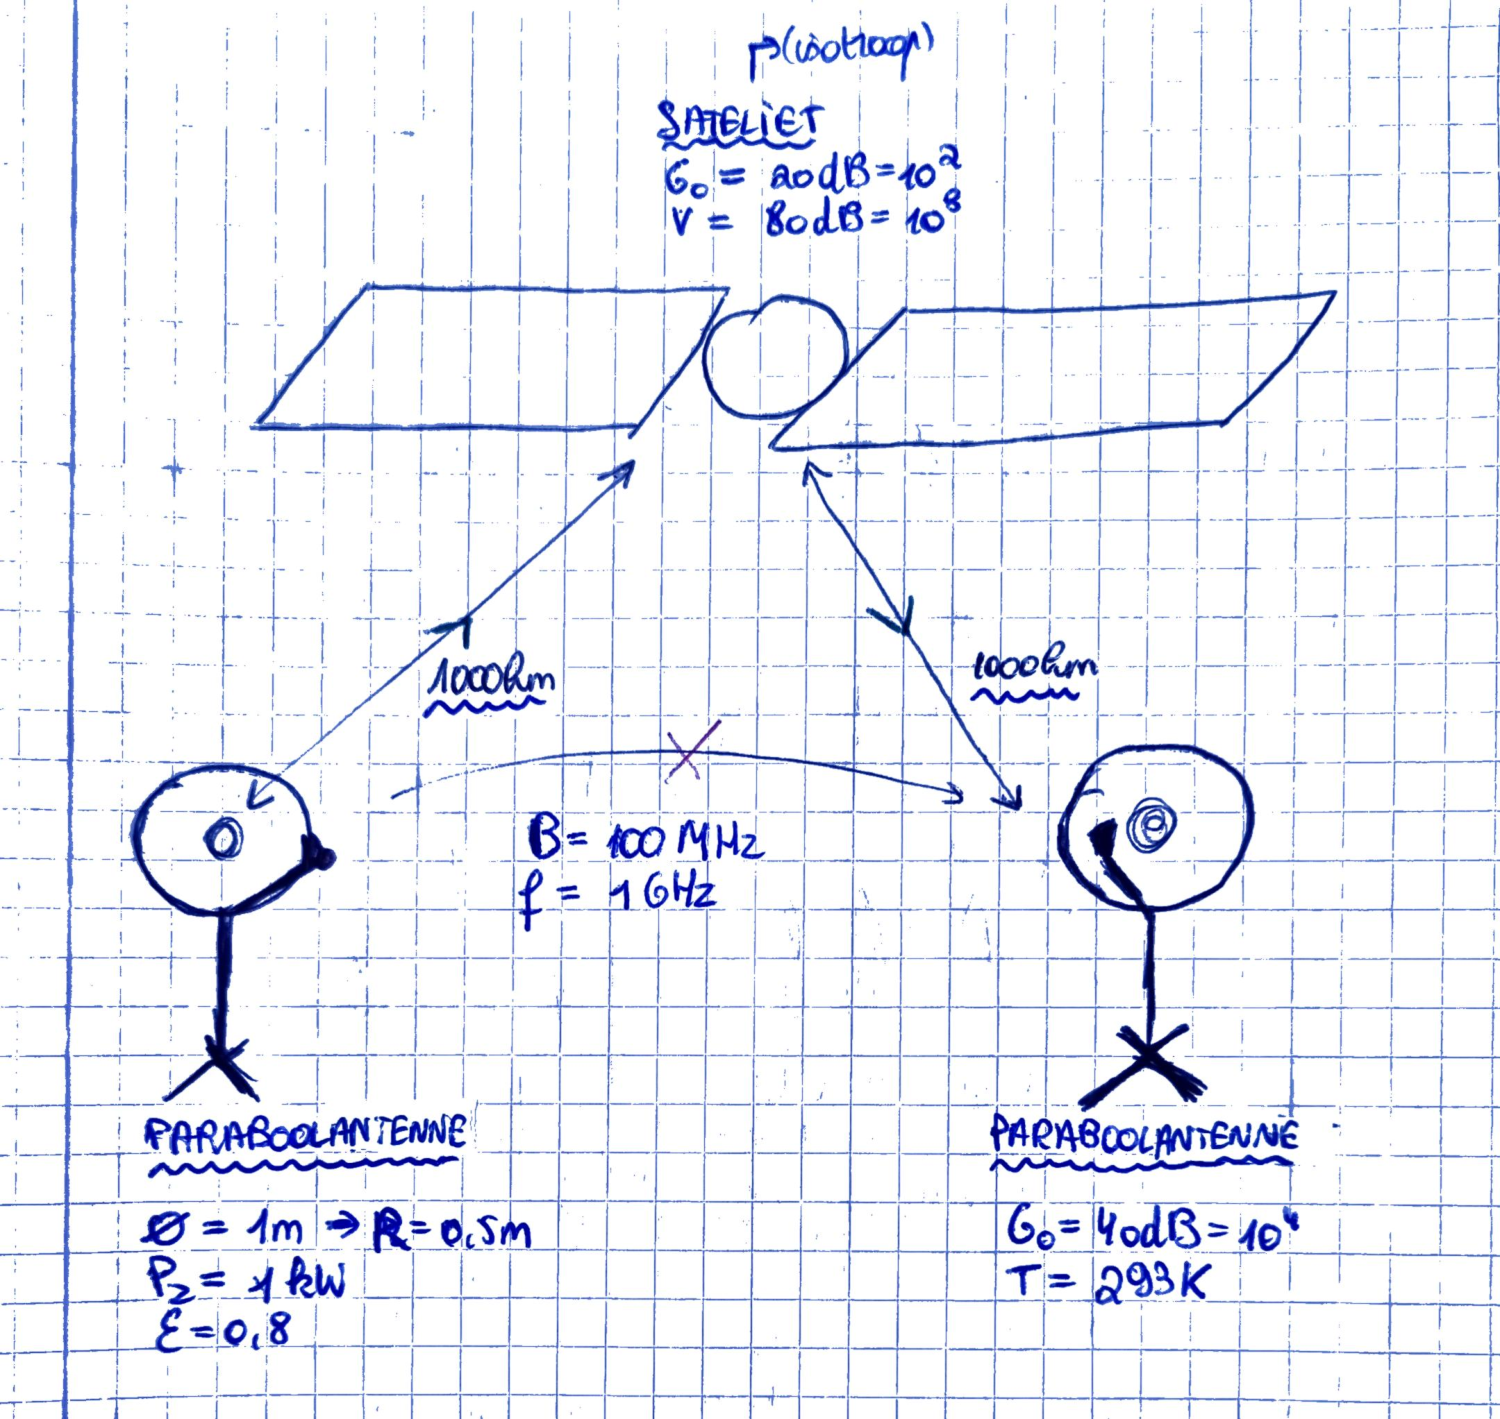
\includegraphics[width=.68\textwidth]{satelliet}
		\caption{Een schets van de gegevens.}
		\label{fig:satelliet}
	\end{figure}

	Er is gevraagd of de huidige infrastructuur voldoende is om alle informatie (\SI{3.6}{\tera\biti}) in de gewenste tijd van één uur = 3600 seconden over te kunnen brengen. We moeten dus controleren of
	\begin{equation}
		\label{shannon}
		C \geq \frac{\SI{3.6}{\tera\biti}}{\SI{3600}{\second}} \qquad \overset{\text{Shannon}}{\Longleftrightarrow} \qquad B \cdot \log_2\left(1+\frac{P_o}{P_n}\right) \geq \SI{1}{\giga\biti\per\second}
	\end{equation}

	We berekenen het ontvangen vermogen in de satelliet.

	\underline{\textbf{Merk op}} dat \(R\neq r\)! \(R_1=R_2\) is de afstand tussen de paraboolantenne en de satelliet (zelfde voor beide satellieten, namelijk 1000 km) en \(r_{p_1}\) is de straal van de verzendende paraboolantenne.
	\begin{align*}
		P_{o,s} &= \text{(vermogensdichtheid bij straling)}_{p_1} \cdot \text{(effectief oppervlak)}_s \\
		&= p_{p_1}(\theta,\phi,R_1) \cdot A_{e,o,s}(\theta, \phi)\\
		&= \left(\frac{P_{z,p_1}}{4\pi R_1^2}\cdot \underbrace{G_{z,p_1}(\theta,\phi)}_\downarrow \right)\cdot \left(\frac{\lambda^2}{4\pi}\cdot G_{o,s}(\theta, \phi)\right) \\
		&= \frac{P_{z,p_1}}{4\pi R_1^2}\cdot \overbrace{ \underbrace{A_{e,z,p_1}(\theta,\phi)}_\downarrow\cdot \cancel{\frac{4 \pi}{\lambda^2}} } \cdot \cancel{\frac{\lambda^2}{4\pi}}\cdot G_{o,s}(\theta, \phi) \\
		&= \frac{P_{z,p_1}}{4\cancel{\pi} R_1^2}\cdot \overbrace{ \varepsilon_{p_1} \cdot \cancel{\pi} r_{p_1}^2 } \cdot G_{o,s}(\theta, \phi) \\
		&= \SI{5e-9}{\watt} = \SI{5}{\nano\watt}
	\end{align*}
	Vervolgens berekenen we het ontvangen vermogen van de ontvangende paraboolantenne. De satelliet is een isotrope straler, dus de vermogensdichtheid hangt enkel af van \(R\), m.a.w. er is geen sprake van winst.
	\begin{align*}
		P_{o,p_2} &= \text{(vermogensdichtheid bij straling)}_s \cdot (\text{versterking})_s \cdot \text{(effectief oppervlak)}_{p_2} \\
		&= p_{s}(R_2) \cdot V_s \cdot A_{e,o,p_2}(\theta, \phi)\\
		&= \left(\frac{P_{o,s}}{4\pi R_2^2} \right) \cdot V_s \cdot \left(\frac{\lambda^2}{4\pi}\cdot G_{o,p_2}(\theta, \phi)\right) \qquad \qquad \text{met } \lambda = \frac{c}{f} \\
		&= \frac{P_{o,s}}{4\pi R_2^2} \cdot V_s \cdot \frac{c^2}{4\pi f^2}\cdot G_{o,p_2}(\theta, \phi) \\
		&= \SI{2.8497e-12}{\watt} \numberthis \label{ontvangen_vermogen}
	\end{align*}

	Het ontvangen ruisvermogen bij de ontvangende paraboolantenne bedraagt
	\begin{align*}
		P_{n,p_2} &= N_0 \cdot B \\
		&= k \cdot T \cdot B \\
		&= 1.38 \cdot 10^{-23} \unit{\joule\per\kelvin} \cdot \SI{293}{K} \cdot \SI{100e6}{\hertz}\\
		&= \SI{4.0434e-13}{W} \numberthis \label{ruisvermogen}
	\end{align*}

	Als we nu de gegeven bandbreedte van \(B=\SI{100}{\mega\hertz}\) en onze uitkomsten \eqref{ontvangen_vermogen} en \eqref{ruisvermogen} invullen in de formule van Shannon \eqref{shannon}, vinden we dat de capaciteit van het ongeleide fysische transmissiekanaal gelijk is aan \begin{align*}
		C &= B \cdot \log_2\left(1+\frac{P_{o,p_2}}{P_{n,p_2}}\right) \\
		&= \SI{100}{\mega\hertz} \cdot \log_2\left(1+\frac{\SI{2.8497e-12}{\watt}}{\SI{4.0434e-13}{W}}\right) \\
		&= \SI{301}{\mega\biti\per\second} \\
		&= \boxed{\SI{0.301}{\giga\biti\per\second} \leq \SI{1}{\giga\biti\per\second}}
	\end{align*}

	We zien dus dat de huidige infrastructuur \underline{onvoldoende} is om alle informatie in de gewenste tijd over te kunnen brengen. We bekijken nu de aanpassingen die zouden kunnen gebeuren aan de infrastructuur om alsnog binnen één uur tijd de gewenste hoeveelheid informatie door te sturen. We beginnen bij de \underline{goedkoopste \textit{upgrade}}, aangezien we geen dure aanpassing moeten aanschaffen indien we de klus al kunnen klaren met een goedkopere aanpassing:\begin{itemize}
		\item We berekenen eerst hoeveel het ontvangen vermogen in de satelliet precies moet bedragen opdat de capaciteit van het fysisch kanaal groter of gelijk is aan \(\SI{1}{\giga\biti\per\second}\):
		\begin{align*}
				C \geq \SI{1}{\giga\biti\per\second} &\Longleftrightarrow& B \cdot \log_2\left(1+\frac{P_{o,p_2}}{P_{n,p_2}}\right)& \geq \rood[\SI{1e9}{\biti\per\second}] \\
				&\Longleftrightarrow& \log_2\left(1+\frac{P_{o,p_2}}{P_{n,p_2}}\right)& \geq \frac{10^9}{B} \\
				&\Longleftrightarrow& \left(1+\frac{P_{o,p_2}}{P_{n,p_2}}\right)& \geq 2^{10^9/B} \\
				&\Longleftrightarrow& P_{o,p_2}& \geq P_{n,p_2}(2^{10^9/B}-1) \\
				&\Longleftrightarrow& \frac{P_{o,s}}{4\pi R_2^2} \cdot V_s \cdot \frac{c^2}{4\pi f^2}\cdot G_{o,p_2}& \geq \SI{4.136e-10}{\watt} \numberthis \label{voorwaarde_c}
		\end{align*}
		\item \underline{Optie 3}: Een verhoging van de winst \(G_{o,p_2}\) van de ontvangstantenne kost 1000 euro per extra dB. We voldoen aan voorwaarde \eqref{voorwaarde_c} a.s.a.
		\begin{align*}
			\frac{P_{o,s}}{4\pi R_2^2} \cdot V_s \cdot \frac{c^2}{4\pi f^2}\cdot G_{o,p_2}& \geq \SI{4.136e-10}{\watt} \\
			& \Updownarrow \\
			G_{o,p_2} & \geq \frac{\SI{4.136e-10}{\watt}}{\frac{P_{o,s}}{4\pi R_2^2} \cdot V_s \cdot \frac{c^2}{4\pi f^2}} \\
			& \Updownarrow \\
			G_{o,p_2} & \geq \SI{1.451541e6}{} \\
					& = 10 \cdot \log_{10}(\SI{1.451541e6}{}) \,\unit{\decibel}\\
					& = \SI{61.62}{\decibel}
		\end{align*}
		We zien dus dat we de winst van de antenne met \boxed{\SI{21.62}{\decibel}} moeten verhogen, wat overeenkomt met een kost van \boxed{21 620 \text{ euro}}.

		\newpage
		\item \underline{Optie 2:} Een vergroting van de zendantenne kost ons 2000 euro per extra meter diameter. \\We voldoen aan voorwaarde \eqref{voorwaarde_c} a.s.a.
		\begin{align*}
			\frac{P_{o,s}}{4\pi R_2^2} \cdot V_s \cdot \frac{c^2}{4\pi f^2}\cdot G_{o,p_2}& \geq \SI{4.136e-10}{\watt} \\
			& \Updownarrow \\
			P_{o,s} &\geq \frac{\SI{4.136e-10}{\watt} \cdot (4\pi)^2 \cdot R_2^2 \cdot f^2}{V_s \cdot c^2 \cdot G_{o,p_2}} \\
			& \Updownarrow \\
			\frac{P_{z,p_1}}{4 R_1^2}\cdot \varepsilon_{p_1} \cdot  r_{p_1}^2 \cdot G_{o,s} &\geq \frac{\SI{4.136e-10}{\watt} \cdot (4\pi)^2 \cdot R_2^2 \cdot f^2}{V_s \cdot c^2 \cdot G_{o,p_2}} \\
			& \Updownarrow \\
			r_{p_1}^2 &\geq \frac{\SI{4.136e-10}{\watt} \cdot (4\pi)^2 \cdot R_2^2 \cdot f^2 \cdot 4R_1^2}{V_s \cdot c^2 \cdot G_{o,p_2} \cdot P_{z,p_1} \cdot \varepsilon_{p_1} \cdot G_{o,s} } \\
			& \Downarrow \\
			r_{p_1} &\geq \sqrt{\SI{36.285}{\meter^2}} \\
			&= \SI{6.024}{\meter}\\
			& \Updownarrow \\
			d_{p_1} &\geq \SI{12.05}{\meter}
		\end{align*}
		We hebben dus \SI{11.05}{\meter} extra diameter nodig om aan de capaciteitsvoorwaarde te voldoen. De kost voor deze aanpassing bedraagt \(11.05 \cdot 2000 = \boxed{22 100 \text{ euro}}\).

		\item \underline{Optie 1}: Een vergroting van de bandbreedte naar oneindig kost 20000 euro. We berekenen de capaciteit \(C\) voor \(B \to \infty\): \begin{align*}
			\lim_{B\to\infty} C &= 1.4427 \cdot \frac{P_{o,p_2}}{N_{o,p_2}}\\
			&= 1.4427 \cdot \frac{P_{o,p_2}}{k \cdot T}\\
			&= 1.4427 \cdot \frac{\SI{2.8497e-12}{\watt}}{\SI{1.38e-23}{\joule/\kelvin}
				 \cdot \SI{293}{\kelvin}}\\
			&= \SI{1016783447}{\biti\per\second}\\
			&\approx \SI{1.017}{\mega\biti\per\second}\\
			&\geq \SI{1}{\mega\biti\per\second}
		\end{align*}
	\end{itemize}

	We kiezen er dus voor om de winst van de ontvangstantenne te verhogen (optie 3), aangezien dit de goedkoopste manier is om een capaciteit van minstens \SI{1}{\mega\biti\per\second} te bewerkstelligen.

	\newpage
	\section{Doorlaatbandtransmissie}

	We bekijken internettoegang via een geostationaire satelliet die we ontvangen met een paraboolantenne met een diameter van \SI{60}{\centi\meter} (efficiëntie van de antenne is \(\epsilon=0.8\)). Het zendvermogen aan boord van de satelliet is \SI{100}{\watt}, de winst van de satellietantenne in de richting van de ontvangantenne op de grond is \SI{20}{\decibel}; de afstand tussen satelliet en ontvangantenne is \SI{40000}{\kilo\meter}; de draaggolffrequentie is \SI{10}{\giga\hertz}; de antenneruistemperatuur van de ontvangantenne op de grond is \SI{50}{\kelvin}.

	We bekijken het downloaden van informatie van de satelliet naar de ontvangantenne en wensen een transmissiedebiet van \SI{5}{\mega\bit/\second}. We kiezen voor een QAM-modulatietechniek en een golfvorm met factor \(\alpha=1\); we wensen de kans op foutieve ontvangst van een golfvorm kleiner te houden dan \SI{4e-9}{}.

	\hfill \\
	\underline{Gevraagd:}
	\begin{enumerate}
		\item Bereken de verhouding van de hoeveelheid energie per bit to.v. de ruisvermogendichtheid.
		\item Hoe groot zijn de pakketjes van bits?
	\end{enumerate}

	\hfill \\
	\underline{Oplossing:}
	\begin{enumerate}
		\item We moeten de verhouding tussen de hoeveelheid energie per bit \(E_b\) en de ruisvermogensdichtheid \(N_o\) in de ontvangende paraboolantenne \(p\) berekenen. Deze verhouding is gelijk aan \begin{equation}
			\frac{E_b}{N_o} \label{verhouding}
		\end{equation} Nu geldt voor de \underline{hoeveelheid energie per bit \(E_b\)} dat \begin{equation}
			\left[\frac{\unit{\joule}}{\unit{\bit*}}\right] = \boxed{E_b = \frac{P_o}{r_b}} = \frac{[\unit{\watt}]}{[\unit{\bit/\second}]} = \frac{[\unit{\joule/\second}]}{[\unit{bit/\second}]} \label{hvh_energie}
		\end{equation}

		Merk op dat de \underline{gemiddelde hoeveelheid energie per bit} \(E_b = [\unit{\joule/\bit}]\) \underline{\textbf{niet gelijk is}} aan de \\\underline{energie per \unit{\biti}}, die gegeven wordt door (zie form. juist boven B3): \[W=0.693 \cdot N_o = \left[\unit{\joule\per\biti}\right]\]

		Het transmissiedebiet is gegeven en bedraagt \(r_b=\SI{5}{\mega\bit/\second}=\SI{5e6}{\bit/\second}\).\\ Gebruikmakend van de radiovergelijking, berekenen we dat \begin{align*}
			P_{o,p} &= p(\theta,\phi,R) \cdot A_{e,s}(\theta,\phi) \\
			&= \left(\frac{P_{z,s}}{4\pi R^2} \cdot G_{z,s}(\theta,\phi) \right) \cdot \left( \epsilon_p \cdot r_p^2 \pi \right) \\
			&= \left(\frac{\SI{100}{\watt}}{4\pi \cdot (\SI{40000e3}{\meter})^2} \cdot 10^2 \right) \cdot \left( 0.8 \cdot (\SI{0.3}{\meter})^2 \pi \right) \\
			&= \SI{1.125e-13}{\watt}
		\end{align*}
		Als we nu de waarden voor \(r_b\) en \(P_{o,p}\) invullen in \eqref{hvh_energie}, vinden we dat \begin{equation*}
			E_b = \frac{\SI{1.125e-13}{\watt}}{\SI{5e6}{\bit/\second}} = \SI{2.25e-20}{\joule\per\bit}
		\end{equation*} Dit resultaat substitueren we samen met \(N_o = k\cdot T \) in \eqref{verhouding} en zo vinden we de gevraagde verhouding: \begin{equation*}
		\frac{E_b}{N_o} = \frac{\SI{2.25e-20}{\joule/\bit}}{\SI{1.38e-23}{\joule/\kelvin}\cdot\SI{50}{\kelvin}} = \boxed{32.61}
		\end{equation*}

		\item Er wordt gevraagd om de \underline{grootte \(n_s\) van de pakketjes van bits} te berekenen.

		Het aantal golfvormen voor onze doorlaatbandtransmissie bedraagt \(M=2^n\). Er is gegeven dat er wordt gekozen voor een QAM-modulatietechniek. Voor deze techniek kunnen we de symboolfoutkans \(P_g\) berekenen. Deze mag volgens de opgave ten hoogste \SI{4e-9}{} bedragen: \begin{equation*}
			P_g \leq 4 \cdot Q\left(\sqrt{\frac{3\cdot \log_2 M}{M-1}\cdot\frac{E_b}{N_o}}\right) \, \text{(formularium)} \qquad \qquad P_g \leq \SI{4e-9}{} \, \text{(gegeven)}
		\end{equation*}

		We berekenen dat dus moet gelden dat \begin{align*}
			\SI{4e-9}{} \geq 4 \cdot Q\left(\sqrt{\frac{3\cdot \log_2 M}{M-1}\cdot 32.6}\right) &\overset{M=2^n}{\Longleftrightarrow} 10^{-9} \geq Q\left(\sqrt{\frac{3\cdot \log_2 2^n}{2^n-1}\cdot 32.6}\right) \\
					&\overset{\text{form.}}{\Longleftrightarrow} 6 \rood[\leq] \sqrt{\frac{3n}{2^n-1}\cdot 32.6} \\
					&\Longrightarrow 36 \leq \frac{3n}{2^n-1}\cdot 32.6\\
					&\Longleftrightarrow \boxed{1.1043 \leq \frac{3n}{2^n-1}}
		\end{align*}

		Als we nu een paar waarden voor \(n\) invullen, zien we dat moet gelden dat \(n \leq 3\).\\
		We kiezen \(n\) zo \underline{groot mogelijk}, dus \(\boxed{n=3}\)

		Waarom zo groot mogelijk? Omdat er in doorlaatband geldt dat \begin{equation*}
			r_b = n_s \cdot r_s \Leftrightarrow r_s = \frac{r_b}{n_s}, \qquad B = 2(1+\alpha)f_m, \qquad T_s = \frac{1}{2f_m}=\frac{1}{r_s} \Leftrightarrow f_m = \frac{1}{2}r_s
		\end{equation*} Hieruit volgt: \begin{equation*}
			B = \cancel{2}(1+\alpha)\cdot \frac{1}{\cancel{2}}r_s = (1+\alpha)\cdot \frac{r_b}{n_s}
		\end{equation*}

		We zien dus dat voor een gegeven transmissiebitrate \(r_b\), de bandbreedte zal \underline{dalen} bij stijgende \(n_s=n=\) aantal bits per pakket (of per verzonden symbool/golfvorm). Of omgekeerd: voor een gegeven bandbreedte \(B\) kunnen we \(r_b\) toch nog opdrijven door \(n_s\) groter te maken.

		Maar er staat een beperking op: we kunnen niet zo maar oneindig de bitrate opdrijven en onder de beperkte bandbreedtelimiet blijven: hoe meer golfvormen we namelijk versturen, hoe meer verschillende amplitudes we versturen, hoe kleiner het verschil tussen de amplitudes, en uiteindelijk hoe moeilijker voor de ontvanger om de verschillende amplitudes van elkaar te onderscheiden. Bij heel hoge \(n_s\) hebben we dus een grote kans om golfvormen foutief te onderscheiden aan de ontvangstkant.

		QAM (\textit{Quadrature Amplitude Modulation}) voert amplitude modulatie uit op zowel een sinusgolf als een cosinusgolf, beiden met dezelfde draaggolffrequentie \(f_c\).

	\end{enumerate}

	\newpage
	\section{Multiplexing}

	Een digitaal signaal met een transmissiedebiet van \SI{80}{\kilo\bit/\second} wordt in basisband verstuurd met
	QAM-16 modulatie. Voor de golfvorm wordt een factor \(\alpha = 0.5\) gebruikt.

	\hfill \\
	\underline{Gevraagd}:
	\begin{enumerate}
		\item Bepaal de vereiste bandbreedte.
		\item Een aantal dergelijke signalen worden nu met FDM verstuurd in de band van 140-240 kHz. We gebruiken enkel-zijband-modulatie waarbij de onderste zijband wordt behouden. Hoeveel signalen kunnen er maximaal worden gemultiplext?
		\item Wat zijn de draaggolffrequenties als we zorgen voor maximale spreiding in de band 140-240 kHz?
		\item Teken het spectrum.
	\end{enumerate}

	\hfill \\
	\underline{Oplossing}:
	\begin{enumerate}

		\item We moeten de bandbreedte \(B\) berekenen.

		Er is gegeven dat het transmissiedebiet gelijk is aan \(r_b = \SI{80e3}{\bit/\second}\).

		Bovendien is er gegeven dat we aan QAM-\underline{16} modulatie doen. Dit wil zeggen dat er 16 golfvormen worden gebruikt. We kunnen hieruit het aantal bits per pakket (of per verzonden symbool/golfvorm) berekenen: \begin{equation*}
			M=16 \quad \Longrightarrow \quad 2^{n_s} =16 \quad \Longrightarrow \quad n_s = \SI{4}{\bit/\symbool}
		\end{equation*} Omdat we \(r_b\) en \(n_s\) kennen, kunnen we berekenen hoeveel symbolen/seconde er worden verzonden: \begin{equation*}
			r_b = n_s \cdot r_s \quad \Longrightarrow \quad n_s = \frac{r_b}{r_s} = \frac{\SI{80e3}{\bit/\second}}{\SI{4}{\bit/\symbool}} = \SI{20e3}{\symbolen/\second} = \SI{20e3}{\underline{\baud}}
		\end{equation*} Nu volgt, door de definitie van de symboolperiode \(T_s\) dat \begin{align*}
		T_s = \frac{1}{r_s} = \frac{1}{2f_m} & \Rightarrow \, r_s = 2f_m\\
		&\Rightarrow \,  f_m = \frac{20 \cdot 10^3}{2}\\
		&\Rightarrow \, f_m = \SI{10}{\kilo\hertz}
		\end{align*}

		We kunnen nu de bandbreedte voor een golfvorm berekenen. Een illustratie van het frequentiespectrum is te zien in Figuur \ref{fig:raised_cosine}. We berekenen dat \[B \overset{\text{basisband}}{=} (1+\alpha)f_m = (1+0.5) \cdot \SI{10}{\kilo\hertz} \quad \Longrightarrow \quad \boxed{B = \SI{15}{\kilo\hertz}}\]

		\begin{figure}[h!]
			\centering
			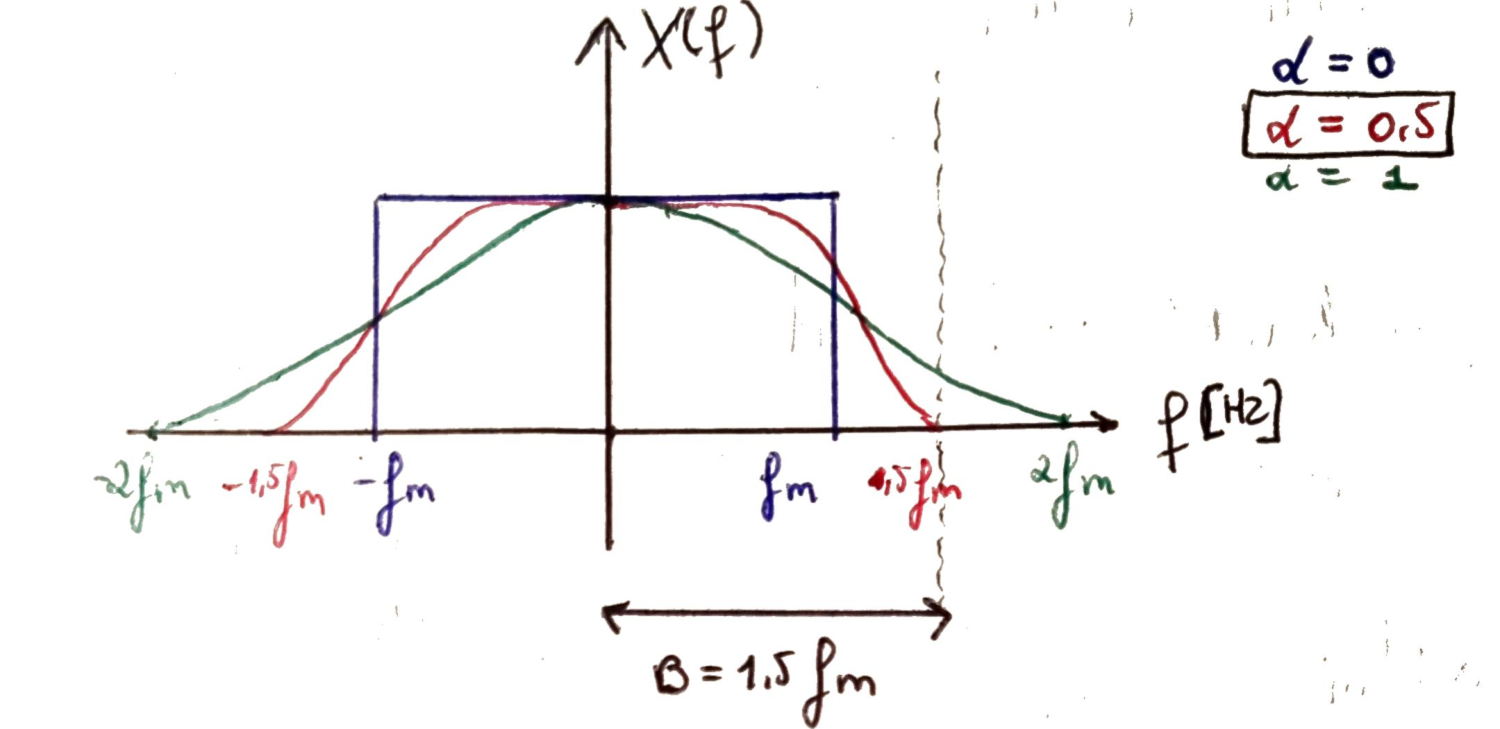
\includegraphics[width=.4\textwidth]{raised_cosine}
			\caption{De frequentie-inhoud \(X(f)\) -- met \textit{raised cosine roll-off} -- van de verzonden golfvorm \(x(t)\)}
			\label{fig:raised_cosine}
		\end{figure}

		\item We berekenen hoeveel signalen er kunnen worden gemultiplext.

		Er is gegeven dat we in doorlaatband de frequenties 140-240 kHz gebruiken. We beschikken dus over een doorlaatbandbreedte van \SI{100}{\kilo\hertz}.

		We maken gebruik van enkel-zij-band-modulatie waarbij de onderste zijband wordt behouden. We gaan er vanuit dat we beschikken over een \textbf{\underline{ideale laagdoorlaatfilter}} en dat we aan de hand van deze filter enkel de frequentie-inhoud voor negatieve frequenties (links van de verticale as) in Figuur \ref{fig:raised_cosine} versturen. Op die manier verbruiken we \SI{15}{\kilo\hertz} per verzonden (halve) golfvorm.

		We zien dus dat we \boxed{\text{6 golfvormen}} van \SI{15}{\kilo\hertz} kunnen verzenden over de beschikbare doorlaatbandbreedte van \SI{100}{\kilo\hertz} tussen \SI{140}{\kilo\hertz} en \SI{240}{\kilo\hertz}.

		\begin{figure}[h!]
			\centering
			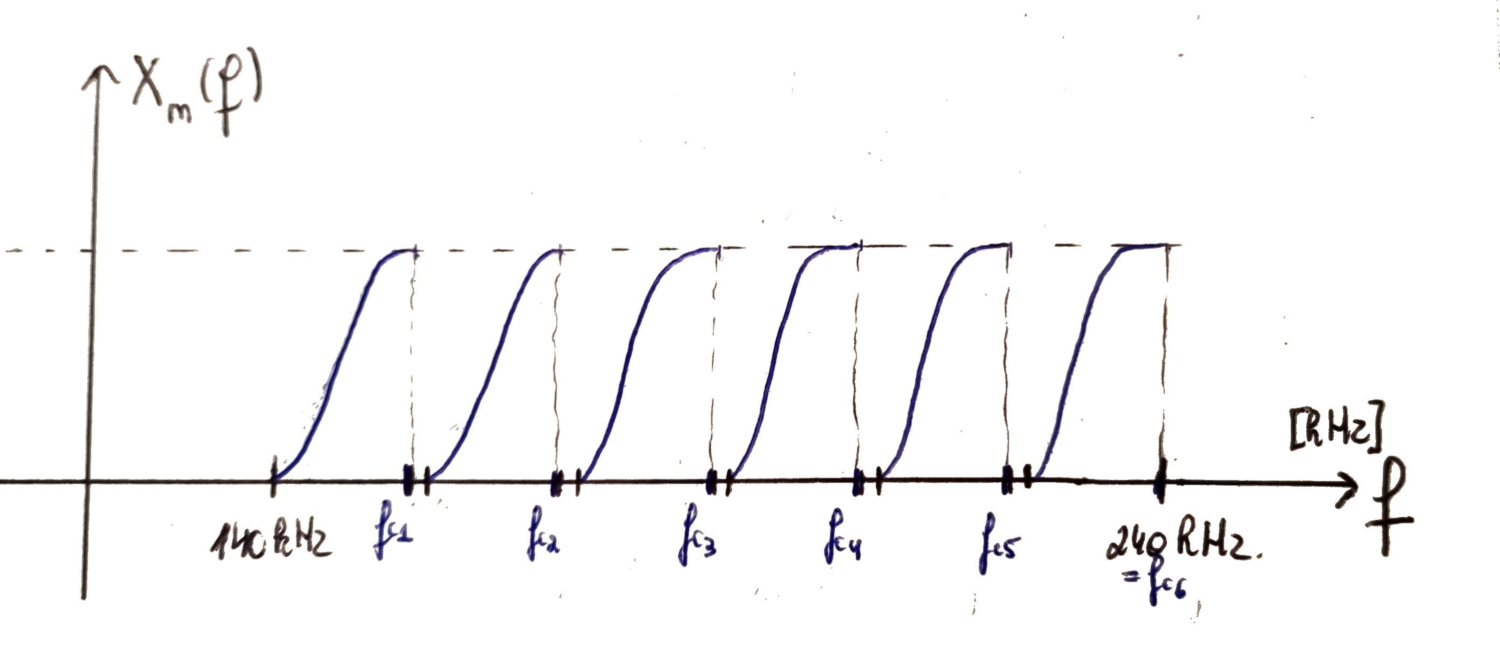
\includegraphics[width=.8\textwidth]{doorlaatspectrum}
			\caption{Het \textbf{(\underline{positieve deel van het})} spectrum van de doorlaatband met de frequentie-inhouden van de verzonden golfvormen. Het negatieve gedeelte bevat exact hetzelfde, maar dan \textbf{\underline{gespiegeld}}.}
			\label{fig:doorlaatspectrum}
		\end{figure}

		\item We bepalen nu de draaggolffrequenties \(f_{c,i}\) (\(i\in\{1,...,6\}\)) voor alle 6 golfvormen, op een manier zó dat er maximale spreiding is. Hiermee bedoelen we dat we de volledige bandbreedte van \SI{140}{\kilo\hertz} tot en met \SI{240}{\kilo\hertz} benutten, maar dat de spreiding tussen de golven binnen dit frequentie-interval zo groot mogelijk is.

		We hebben een \textit{overschot}bandbreedte van \(\SI{100}{\kilo\hertz} - 6 \cdot \SI{15}{\kilo\hertz} = \SI{10}{\kilo\hertz}\). Deze `overschot' verdelen we over de 5 \textit{tussenstukken} tussen de frequentiespectra van de golven. Zo vinden we dat er in het frequentiespectrum van de doorlaatband \(\frac{\SI{10}{\kilo\hertz}}{5} = \SI{2}{\kilo\hertz}\) tussen elke golfvorm zit. Dit wordt geïllustreerd in Figuur \ref{fig:doorlaatspectrum}.

		We kunnen nu de draaggolffrequenties bepalen:
		\begin{table}[h!]
			\centering
			\(\begin{array}{c *{5}{|c}}
				f_{c,1}               & f_{c,2}               & f_{c,3}               & f_{c,4}               & f_{c,5}               & f_{c,6}               \\ \hline
				\SI{155}{\kilo\hertz} & \SI{172}{\kilo\hertz} & \SI{189}{\kilo\hertz} & \SI{206}{\kilo\hertz} & \SI{223}{\kilo\hertz} & \SI{240}{\kilo\hertz}
			\end{array}	\)
		\end{table}

	\end{enumerate}

\end{document}



